\documentclass[prb,12pt]{revtex4-2}

\usepackage{amsmath, amssymb,physics,amsfonts,amsthm}
\usepackage[most]{tcolorbox}
\usepackage{enumitem}
\usepackage{cancel}
\usepackage{booktabs}
\usepackage{polynom}
\usepackage{tabularx}
\usepackage{tikz}
\usepackage{hyperref}
\usepackage{enumitem}
\usepackage{ulem}
\usepackage{transparent}
\usepackage{float}
\usepackage{multirow}
\newtheorem{Theorem}{Theorem}
\newtheorem{Proposition}{Theorem}
\newtheorem{Lemma}[Theorem]{Lemma}
\newtheorem{Corollary}[Theorem]{Corollary}
\newtheorem{Example}[Theorem]{Example}
\newtheorem{Remark}[Theorem]{Remark}
\theoremstyle{definition}
\newtheorem{Problem}{Problem}
\theoremstyle{definition}
\newtheorem{Definition}[Theorem]{Definition}
\newenvironment{parts}{\begin{enumerate}[label=(\alph*)]}{\end{enumerate}}
%tikz
\usetikzlibrary{patterns}
\usetikzlibrary{matrix}
%tcolorbox
\tcbset{breakable=true,toprule at break = 0mm,bottomrule at break = 0mm}
% definitions of number sets
\newcommand{\N}{\mathbb{N}}
\newcommand{\R}{\mathbb{R}}
\newcommand{\Z}{\mathbb{Z}}
\newcommand{\Q}{\mathbb{Q}}
\newcommand{\C}{\mathbb{C}}
\allowdisplaybreaks
\begin{document}
\title{Fortgeschrittene Fehlerrechnung Übungsblatt 3}
	\author{Jun Wei Tan}
	\email{jun-wei.tan@stud-mail.uni-wuerzburg.de}
	\affiliation{Julius-Maximilians-Universit\"{a}t W\"{u}rzburg}
	\date{\today}
	\maketitle

\section{Messung}
\begin{center}
\begin{tabular}{cc}
	\toprule
	\textbf{Temperatur ($^{\circ}$C)} & \textbf{Luftfeuchte (g/m$^3$)} \\\midrule 
-15 & 0,47 \\\midrule
-11 & 0,54 \\\midrule
-7 & 0,79 \\\midrule
-3 & 1,32 \\\midrule
1 & 1,13 \\\midrule
5 & 1,26 \\\midrule
9 & 3,02 \\\midrule
13 & 2,99 \\\midrule
17 & 3,15 \\\midrule
21 & 3,90 \\\midrule
25 & 5,04 \\\midrule
29 & 7,72 \\\midrule
33 & 11,02 \\\midrule
37 & 13,42 \\\midrule
41 & 20,85 \\\bottomrule
\end{tabular}
\end{center}
Im Zukunft werden wir die Temperatur mit $T$ und Luftfeuchte mit $\rho$ bezeichnen.
\section{Kovarianz und Korrelationskoeffizient}
Wir berechnen jetzt die Kovarianz und Korrelationskoeffizient
\begin{align*}
	N=&~15\\
	\bar{T}=&~13~{}^{\circ}\text{C}\\
	\bar{\rho}=&~5,108~\text{gm}^{-3}\\
	\sigma_T=&~\left[\frac 1N\sum (T_i-\bar{T})^2\right]^{1/2}\\
	=&~17,282~{}^{\circ}\text{C}\\
	\sigma_\rho=&~\left[\frac 1N\sum (\rho_i-\bar{\rho})^2\right]^{1/2}\\
	=&~5,6499~\text{gm}^{-3}\\
	\text{Kovarianz }\sigma_{T\rho}=&~\frac 1N \sum (T_i-\bar{T})(\rho_i - \bar{\rho})\\
	=&~83,688~{}^{\circ}\text{Cgm}^{-3}\\
	\text{Korrelationskoeffizient }r=&~\frac{\sigma_{T\rho}}{\sigma_T\sigma_\rho}\\
	=&~0,857095
\end{align*}
Laut Tabelle (Taylor) ist die Wahrscheinlichkeit, bei 15 nicht korrelierten Messwerte ein $|r|>0,8$ zu bekommen kleiner als $0,05\%$. Weil $0,85$ großer als $0,8$ ist, ist die Messung hochsignifikant.
\section{Regression}
Das Ziel ist eine Best-Fit Gerade
\[\rho = a+ bT\]
zu finden. Dafür brauchen wir die Annahme, dass der Fehler in $T$ vernachlässigbar im Vergleich zum Fehler in $\rho$ ist. Der Messfehler eines marktüblichen Thermometers ist 0,1 $^\circ$C, und die Fehler der Instrumenten im Umweltstation sind wahrscheinlich deutlich kleiner. Daher ist der Fehler in $T$ wahrscheinlich vernachlässigbar.

Außerdem brauchen wir, dass die Messwerte voneinander statistisch unabhängig sind. Die Annahme ist wahrscheinlich richtig, weil die Messungen über das Jahr gemacht werden.

Die Idee zur Berechnung der Regessionswerte ist: Wir suchen $a$ und $b$, sodass der quadratische Fehler
\[\chi^2=\sum_{i=1}^N \left[\frac{\rho_i - a - b T_i}{\sigma_i}\right]^2\]
so klein wie möglich ist. Wir nehmen an, dass alle Datenpunkte den gleichen Fehler haben. Damit können wir die Regressionswerte und deren Fehler mit dem Formel aus VL08 Fehlerrechnung 1 berechnen.
Wir benötigen folgende Größen
\begin{align*}
	\sum T_i=&195{}^{\circ}\text{C}\\
	\sum \rho_i=& 76,72~\text{gm}^{-3}\\
	\sum T_i^2=&7015\left({}^{\circ}\text{C}\right)^2\\
	\sum T_i \rho_i=& 2251,38~{}^{\circ}\text{Cgm}^{-3}
\end{align*}
Danach definieren wir
\begin{align*}
	\Delta =& N\sum T_i^2 - \left(\sum T_i\right)^2\\
	=&67200\left({}^{\circ}\text{C}\right)^2
\end{align*}
Die Koeffizienten werden dann bestimmt durch
\begin{align*}
	a=&\frac 1\Delta \left(\sum T_i^2 \sum \rho_i - \sum T_i \sum T_i \rho_i\right)\\
	=&1,465330357142856~\text{gm}^{-3}\\
	b=& \frac 1\Delta\left(N\sum T_i \rho_i - \sum T_i \sum \rho_i\right)\\
	=& 0,2802053571428572~\text{gm}^{-3}({}^{\circ}\text{C})^{-1}
\end{align*}
Zur Berechnung der Fehler brauchen wir die Stichprobevarianz
\begin{align*}
s^2&=\frac{1}{N-2}\sum \left(\rho_i - a - bT_i\right)^2\\
&\approx 9,77488085164836~\text{g}^2\text{m}^{-6}
\end{align*}
Deren Fehler werden durch
\begin{align*}
\sigma_a =& \left[\frac{s^2}{\Delta}\sum T_i^2\right]^{1/2}\\
\approx& 1,0 ~\text{gm}^{-3}\\
\sigma_b=& \left[N\frac{s^2}{\Delta}\right]^{1/2}\\
=&0,047~\text{gm}^{-3}({}^{\circ}\text{C})^{-1}
\end{align*}
Insgesamt ist
\begin{align*}
	a=&(1,5\pm 1,0)~\text{gm}^{-3}\\
	b=&(0,280\pm 0,047)~\text{gm}^{-3}({}^{\circ}\text{C})^{-1}
\end{align*}
\begin{center}
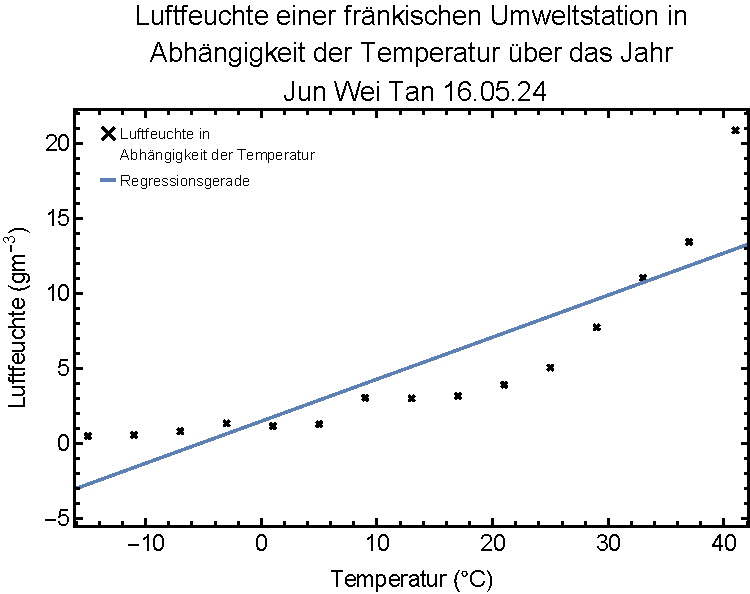
\includegraphics[width=0.7\textwidth]{plt.pdf}
\end{center}
\end{document}
